\chapter{Evaluation}
\label{ch:evaluation}

%Describe the approaches you have used to evaluate that the solution you have designed in \Cref{ch:design} and executed in \Cref{ch:implementation} actually solves the problem identified in \Cref{ch:introduction}.

%While you can discuss unit testing etc. you have carried here a little bit, that is the minimum. You should present data here and discuss that. This might include \emph{e.g.} performance data you have obtained from benchmarks, survey results, or application telemetry / analytics. Tables and graphs displaying this data are good.

\section{数值实验简介}

测试了对于story中问题的两个初始状态，每个求解器在输入步数为1000，10000，100000，1000000的情况下的不同阶数的求解情况，
使用二分法寻找对于固定步长的求解器在10000000步数内的最小cpu时间。
\begin{itemize}
    \item 求解情况在output/track文件夹下，每一行为一个点的坐标。
    \item 对应的maxnorm在output/acc文件夹下，每一行为某阶某求解器在某初值下的误差最大范数和cpu时间。
    \subitem 对于10.191的情况，求误差方法为用同样的求解器求解0到T2/2的解，将其在T2/2的值作为初值，求解T2/2到T2的解，然后利用理查德外推法的公式修正最终解，使用该解与原解计算误差。
    \item 对应最小cpu时间在output/mincpu文件夹下，每一行为某求解器在某初值下的最小cpu时间（对于自适应步长并不生效）。
    \item 对应log在log文件夹下，为命令行输出内容。 
\end{itemize}

\section{部分数值结果展示}
作业中要求的数据生成在output/track1和output/acc1中，其结果如下

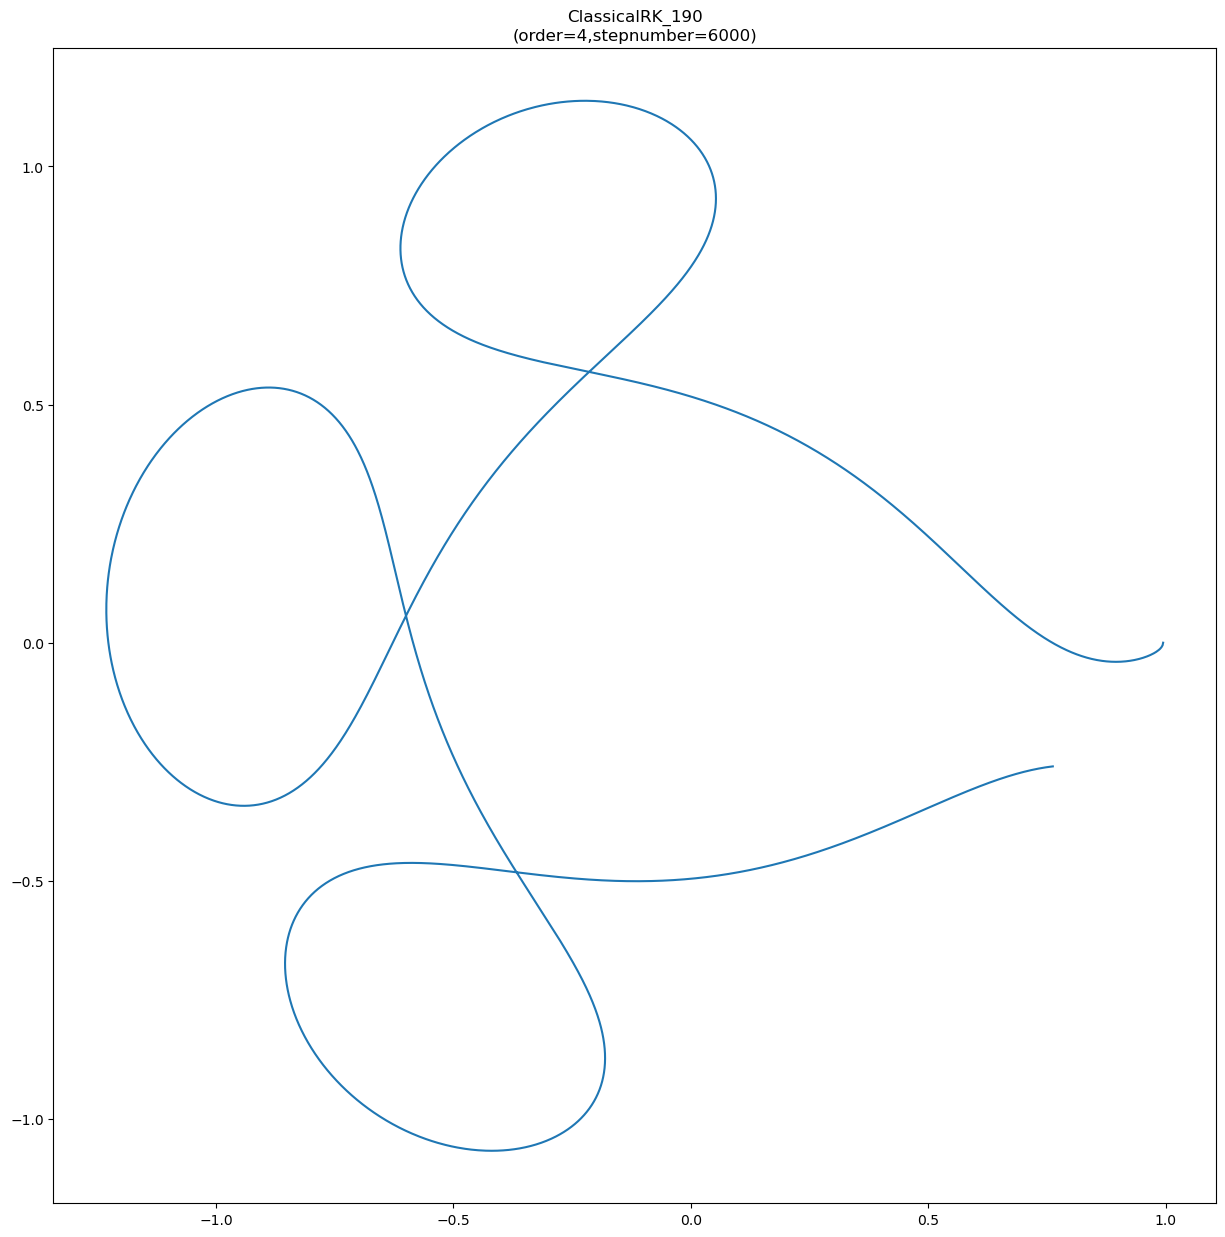
\includegraphics[scale=0.4]{../../img1/track/output_track1_ClassicalRK_190_4.png}

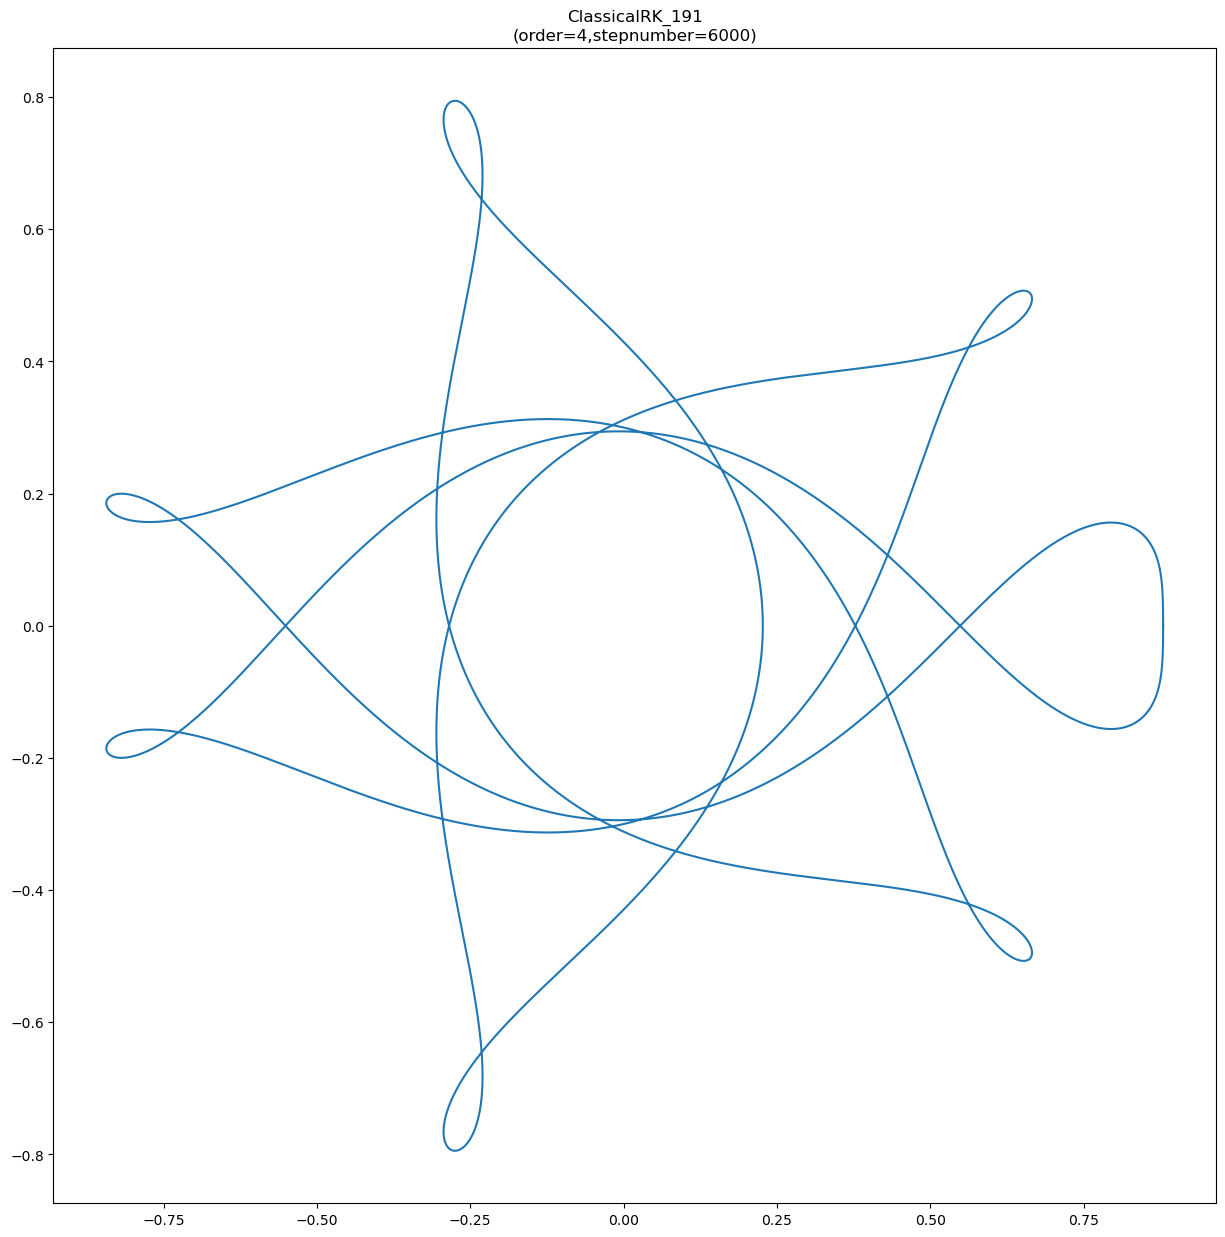
\includegraphics[scale=0.4]{../../img1/track/output_track1_ClassicalRK_191_4.png}

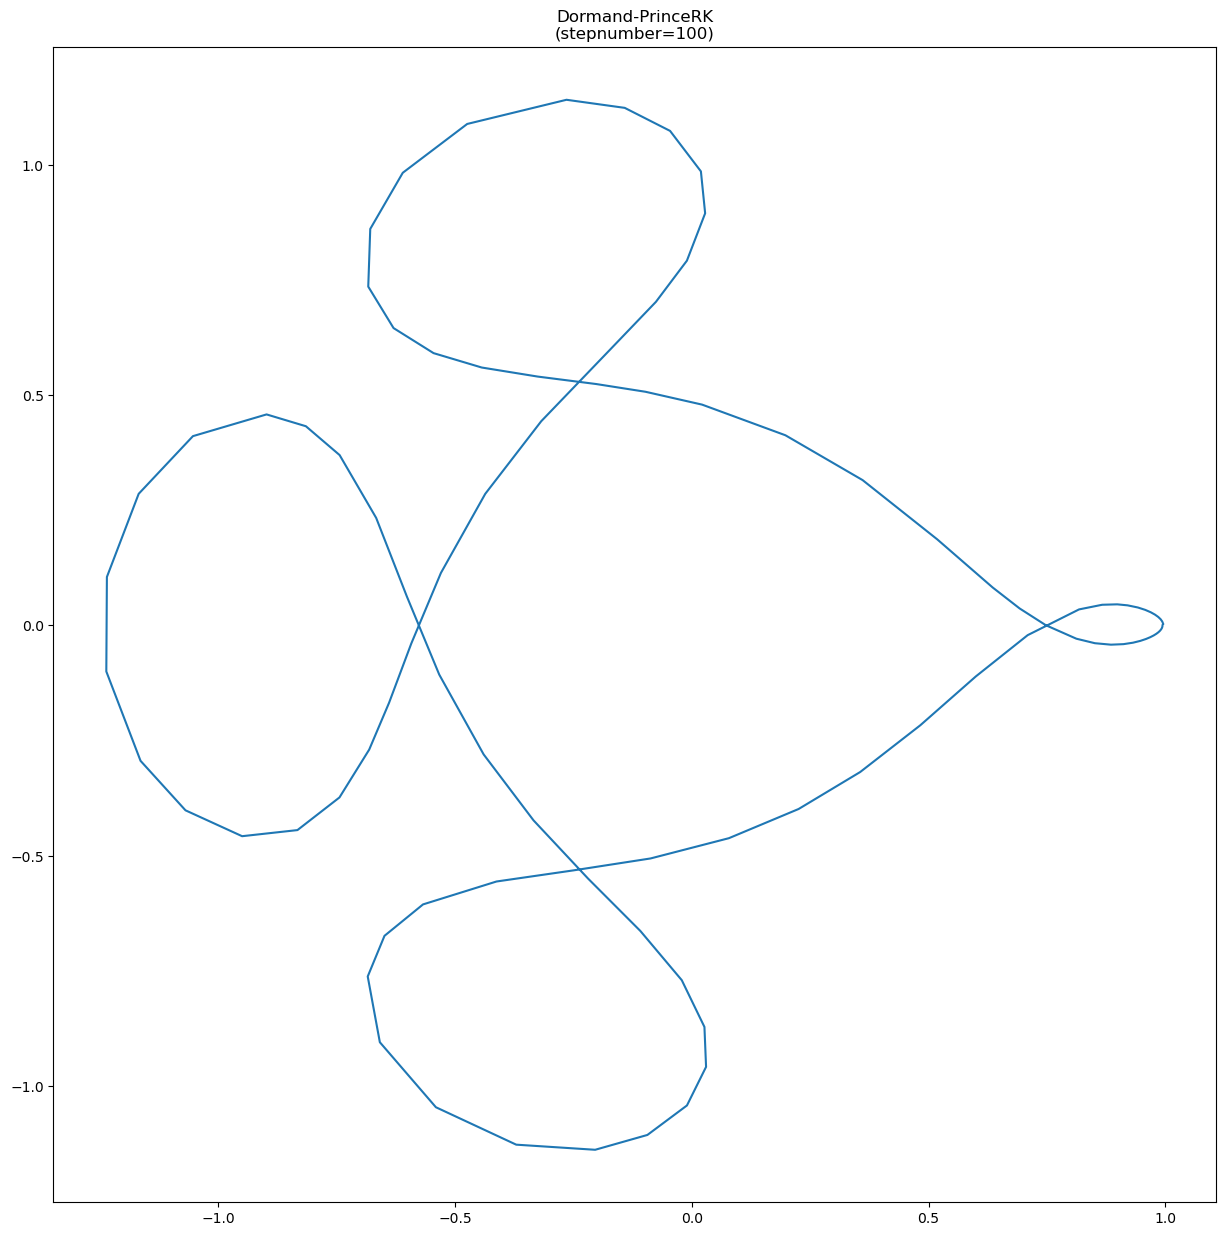
\includegraphics[scale=0.4]{../../img1/track/output_track1_Dormand_PrinceRK_190_5.png}

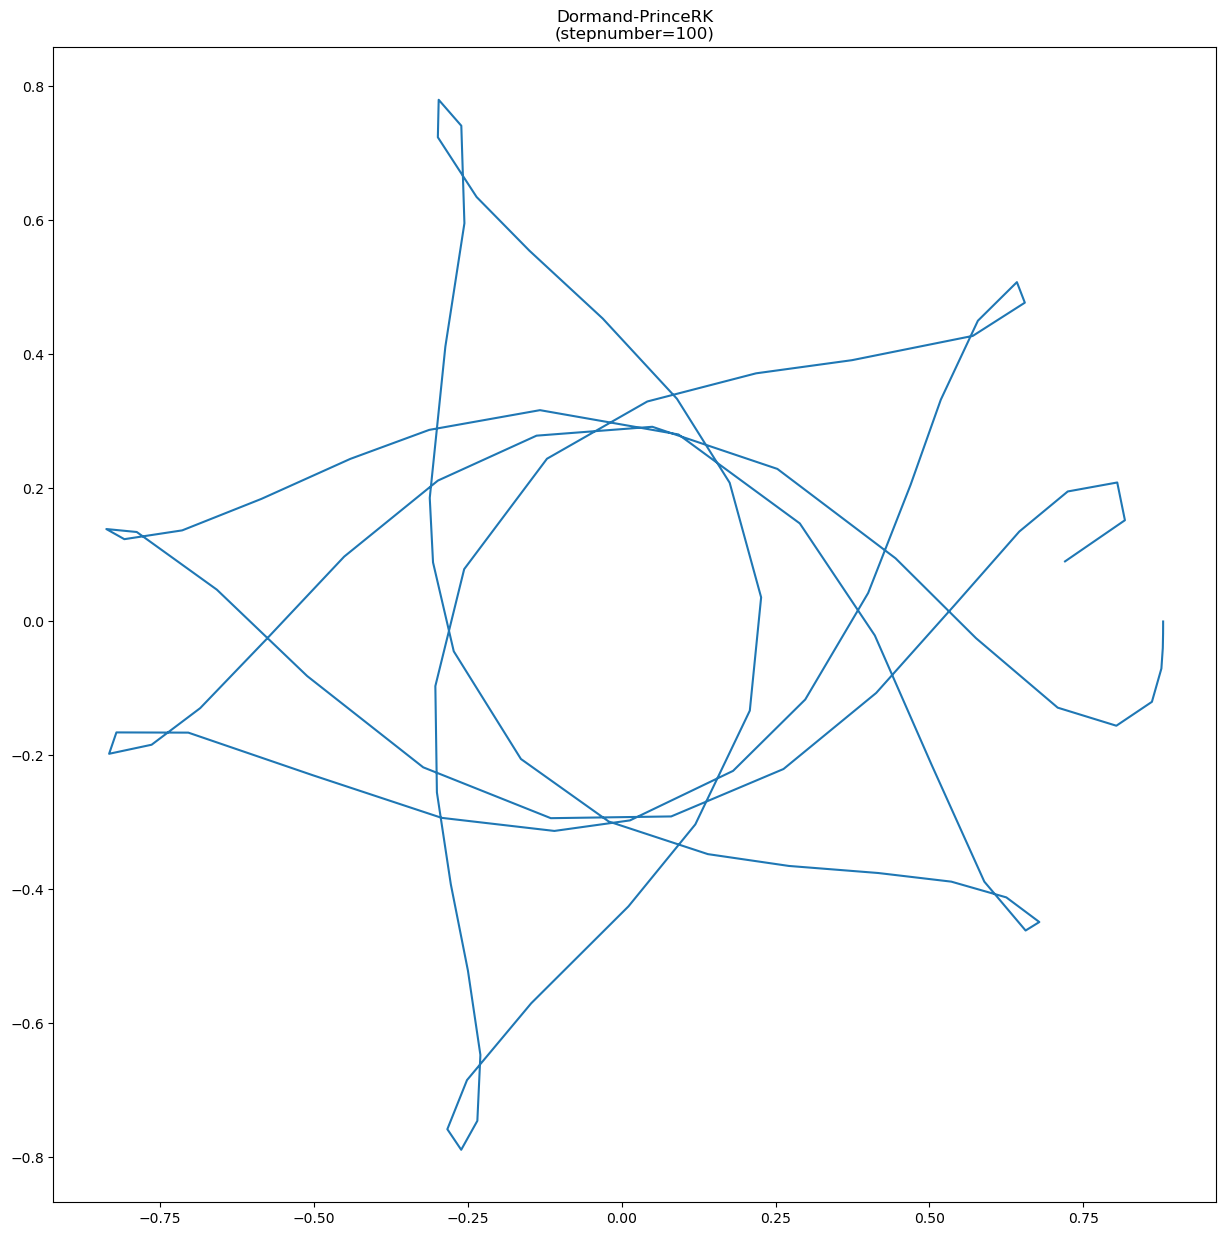
\includegraphics[scale=0.4]{../../img1/track/output_track1_Dormand_PrinceRK_191_5.png}

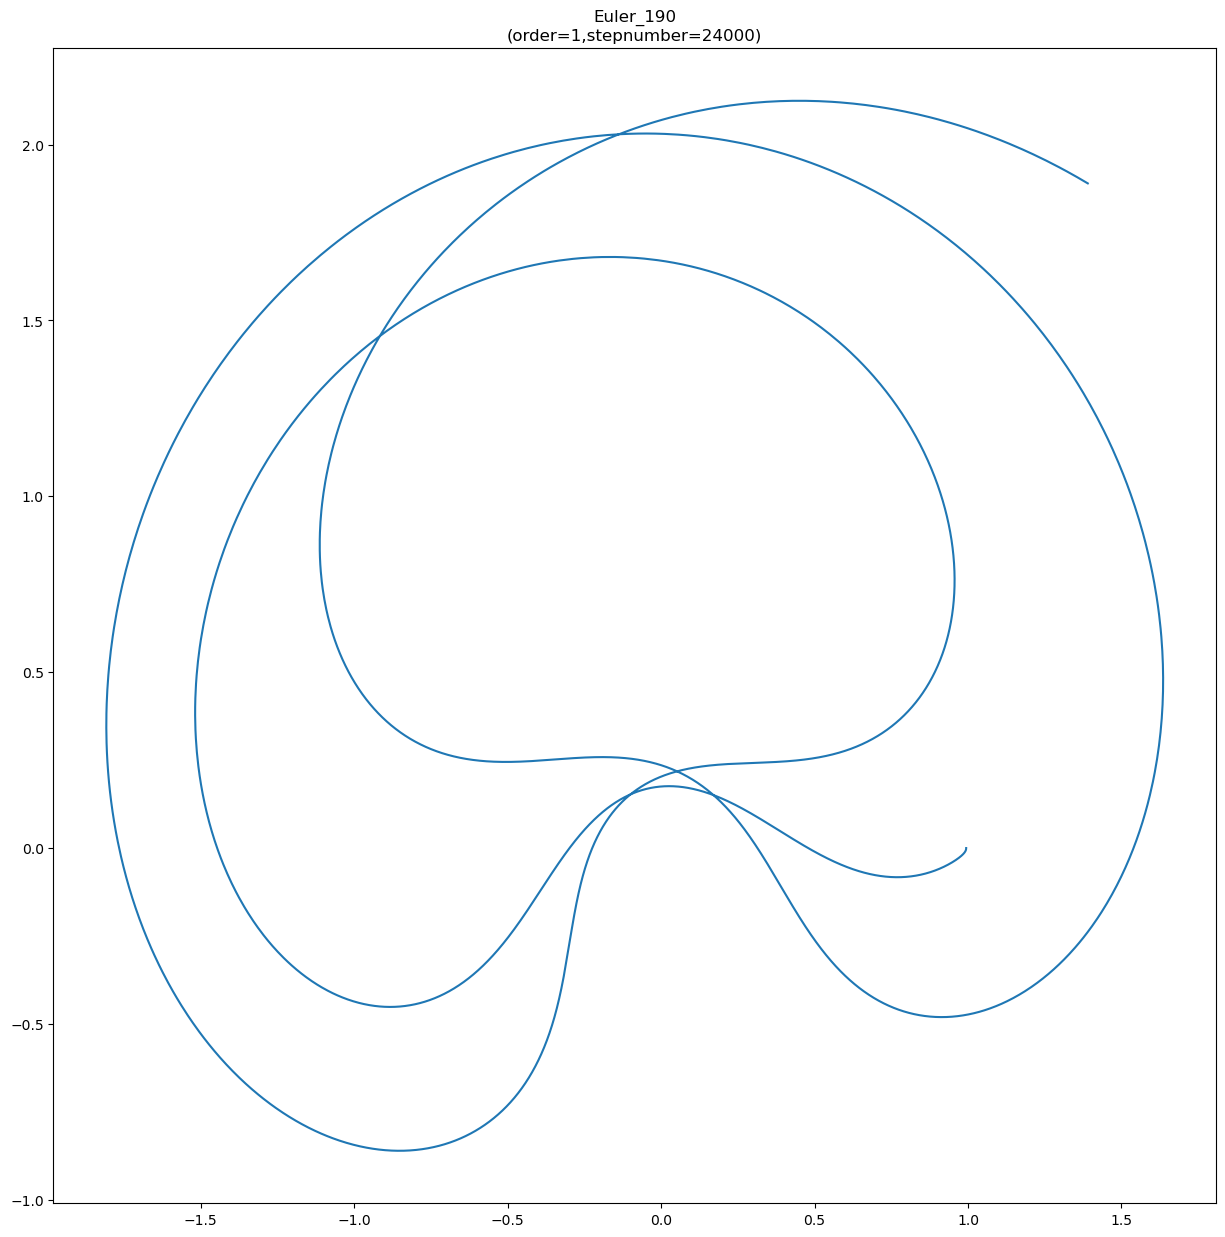
\includegraphics[scale=0.4]{../../img1/track/output_track1_Euler_190_1.png}

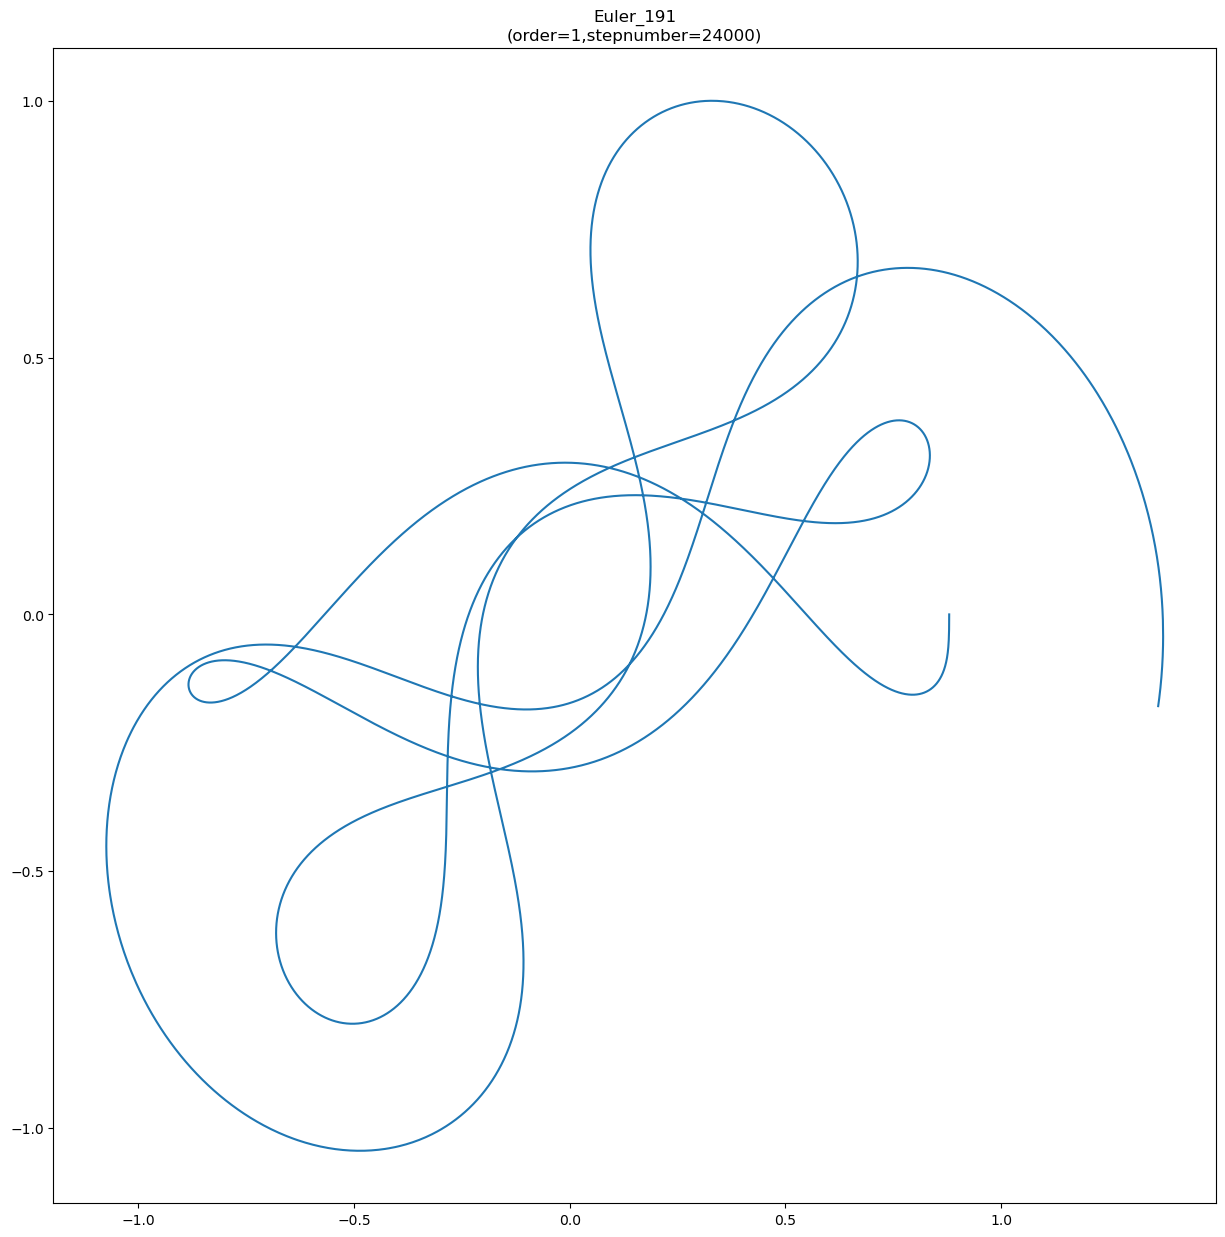
\includegraphics[scale=0.4]{../../img1/track/output_track1_Euler_191_1.png}



\section{最小cpu时间}
使用二分法寻找了使得误差小于0.001的最小cpu时间(最小步数)，结果如下(第一个数据为步数，第二个数据为误差最大范数，第三个数据为cpu时间，为-1,0,0表示没有在10000000步内寻找到):
\begin{itemize}
    \item Adams-Bashforth\_190 (order = 1) : -1 0 0
    \item Adams-Bashforth\_190 (order = 2) : -1 0 0
    \item Adams-Bashforth\_190 (order = 3) : 790037 0.000999998 4.2921 
    \item Adams-Bashforth\_190 (order = 4) : 406561 0.000999995 2.52626 
    \item Adams-Bashforth\_191 (order = 1) : -1 0 0
    \item Adams-Bashforth\_191 (order = 2) : 23895 0.000999962 0.0838745 
    \item Adams-Bashforth\_191 (order = 3) : 16077 0.000999947 0.0832476 
    \item Adams-Bashforth\_191 (order = 4) : 3292 0.000999077 0.0254242 
\end{itemize}

\begin{itemize}
    \item Adams-Moulton\_190 (order = 2) : -1 0 0
    \item Adams-Moulton\_190 (order = 3) : 375851 0.000999999 4.18314 
    \item Adams-Moulton\_190 (order = 4) : 212824 0.000999984 3.03074 
    \item Adams-Moulton\_190 (order = 5) : 92293 0.000999971 1.26825 
    \item Adams-Moulton\_191 (order = 2) : 11902 0.000999938 0.183787 
    \item Adams-Moulton\_191 (order = 3) : 7743 0.000999873 0.126579 
    \item Adams-Moulton\_191 (order = 4) : 1715 0.000997934 0.0400893
    \item Adams-Moulton\_191 (order = 5) : 1750 0.000997853 0.0480614 
\end{itemize}

\begin{itemize}
    \item Backward Differentiation\_190 (order = 1) : -1 0 0 
    \item Backward Differentiation\_190 (order = 2) : -1 0 0 
    \item Backward Differentiation\_190 (order = 3) : 681187 0.000999993 7.17079 
    \item Backward Differentiation\_190 (order = 4) : 352936 0.000999999 3.63705 
    \item Backward Differentiation\_191 (order = 1) : -1 0 0 
    \item Backward Differentiation\_191 (order = 2) : 20144 0.000999938 0.342755 
    \item Backward Differentiation\_191 (order = 3) : 14073 0.00099985 0.20502 
    \item Backward Differentiation\_191 (order = 4) : 3015 0.000998607 0.102383 
\end{itemize}

\begin{itemize}
    \item ClassicalRK\_190 : 85645 0.00099996 0.811399 
    \item ClassicalRK\_191 : 1080 0.000998308 0.0087803 
\end{itemize}

\begin{itemize}
    \item ESDIRK\_190 : 66138 0.000999983 6.72071 
    \item ESDIRK\_191 : 669 0.000998584 0.122715 
\end{itemize}

\begin{itemize}
    \item GLRK\_190 (order = 2) : 59705 0.000999987 2.09739 
    \item GLRK\_190 (order = 3) : 17183 0.000999848 0.962451 
    \item GLRK\_190 (order = 4) : 7470 0.000999249 0.832366 
    \item GLRK\_190 (order = 5) : 4942 0.000998519 1.08603 
    \item GLRK\_190 (order = 2) : 631 0.000995117 0.211923 
    \item GLRK\_190 (order = 2) : 222 0.000452825 0.16272 
    \item GLRK\_190 (order = 2) : 125 0.000304964 1.18271 
    \item GLRK\_190 (order = 2) : 94 0.000654174 0.921698 
\end{itemize}

\begin{itemize}
    \item Euler\_190 : -1 0 0
    \item Euler\_191 : -1 0 0
\end{itemize}

对于自适应步长方法，还没有设计相应的搜索误差小于0.001的最小cpu时间，观察log发现第五个分量
比较难收敛，但是由于其自适应步长的特性，不论初始步长是什么，计算的时间都差不多，而且很快，从结果来看准确率也不错，
不过在我默认的参数（Eabs，Erel，$\rho$，$\rho_{max}$，$\rho_{min}$）下第五个分量的误差比较难收敛于0。

\section{max-norm}

\includegraphics[scale = 0.6]{../../img/order/Adams-Bashforth_190.png}

\includegraphics[scale = 0.6]{../../img/order/Adams-Bashforth_191.png}

\includegraphics[scale = 0.6]{../../img/order/Adams-Moulton_190.png}

\includegraphics[scale = 0.6]{../../img/order/Adams-Moulton_191.png}

\includegraphics[scale = 0.6]{../../img/order/Backward_Differentiation_190.png}

\includegraphics[scale = 0.6]{../../img/order/Backward_Differentiation_191.png}


\includegraphics[scale = 0.6]{../../img/order/ClassicalRK_190.png}


\includegraphics[scale = 0.6]{../../img/order/ClassicalRK_191.png}


\includegraphics[scale = 0.6]{../../img/order/Dormand-PrinceRK_190.png}


\includegraphics[scale = 0.6]{../../img/order/Dormand-PrinceRK_191.png}

\includegraphics[scale = 0.6]{../../img/order/ESDIRK_190.png}

\includegraphics[scale = 0.6]{../../img/order/ESDIRK_191.png}


\includegraphics[scale = 0.6]{../../img/order/Euler_190.png}


\includegraphics[scale = 0.6]{../../img/order/Euler_191.png}

\includegraphics[scale = 0.6]{../../img/order/FehlbergRK_190.png}

\includegraphics[scale = 0.6]{../../img/order/FehlbergRK_191.png}

\includegraphics[scale = 0.6]{../../img/order/GLRK_190.png}

\includegraphics[scale = 0.6]{../../img/order/GLRK_191.png}

观察log发现对固定步长，误差接近及其精度时折现表现得不太符合数据（即点应该在对应阶数附近）。但是在误差较大时，是比较符合的，
所有固定步长的方法，都可以找出一条符合算法阶数的折线（除了GLRK求解10.191的情况，因为误差算出来都很小，感觉主要误差不来自于算法）。

\section{不同求解器及其不同精度的求解情况}

\includegraphics[scale = 0.5]{../../img/track/output_track_Adams-Bashforth_190_1.png}

\includegraphics[scale = 0.5]{../../img/track/output_track_Adams-Bashforth_190_2.png}

\includegraphics[scale = 0.5]{../../img/track/output_track_Adams-Bashforth_190_3.png}

\includegraphics[scale = 0.5]{../../img/track/output_track_Adams-Bashforth_190_4.png}

\includegraphics[scale = 0.5]{../../img/track/output_track_Adams-Bashforth_191_1.png}

\includegraphics[scale = 0.5]{../../img/track/output_track_Adams-Bashforth_191_2.png}

\includegraphics[scale = 0.5]{../../img/track/output_track_Adams-Bashforth_191_3.png}

\includegraphics[scale = 0.5]{../../img/track/output_track_Adams-Bashforth_191_4.png}



\includegraphics[scale = 0.5]{../../img/track/output_track_Adams-Moulton_190_2.png}

\includegraphics[scale = 0.5]{../../img/track/output_track_Adams-Moulton_190_3.png}

\includegraphics[scale = 0.5]{../../img/track/output_track_Adams-Moulton_190_4.png}

\includegraphics[scale = 0.5]{../../img/track/output_track_Adams-Moulton_190_5.png}

\includegraphics[scale = 0.5]{../../img/track/output_track_Adams-Moulton_191_2.png}

\includegraphics[scale = 0.5]{../../img/track/output_track_Adams-Moulton_191_3.png}

\includegraphics[scale = 0.5]{../../img/track/output_track_Adams-Moulton_191_4.png}

\includegraphics[scale = 0.5]{../../img/track/output_track_Adams-Moulton_191_5.png}


\includegraphics[scale = 0.5]{../../img/track/output_track_Backward_Differentiation_190_1.png}

\includegraphics[scale = 0.5]{../../img/track/output_track_Backward_Differentiation_190_2.png}

\includegraphics[scale = 0.5]{../../img/track/output_track_Backward_Differentiation_190_3.png}

\includegraphics[scale = 0.5]{../../img/track/output_track_Backward_Differentiation_190_4.png}

\includegraphics[scale = 0.5]{../../img/track/output_track_Backward_Differentiation_191_1.png}

\includegraphics[scale = 0.5]{../../img/track/output_track_Backward_Differentiation_191_2.png}

\includegraphics[scale = 0.5]{../../img/track/output_track_Backward_Differentiation_191_3.png}

\includegraphics[scale = 0.5]{../../img/track/output_track_Backward_Differentiation_191_4.png}

\includegraphics[scale = 0.5]{../../img/track/output_track_ClassicalRK_190_4.png}

\includegraphics[scale = 0.5]{../../img/track/output_track_ClassicalRK_191_4.png}

\includegraphics[scale = 0.5]{../../img/track/output_track_ESDIRK_190_4.png}

\includegraphics[scale = 0.5]{../../img/track/output_track_ESDIRK_191_4.png}

\includegraphics[scale = 0.5]{../../img/track/output_track_Euler_190_1.png}

\includegraphics[scale = 0.5]{../../img/track/output_track_Euler_191_1.png}

\includegraphics[scale = 0.5]{../../img/track/output_track_FehlbergRK_190_4.png}

\includegraphics[scale = 0.5]{../../img/track/output_track_FehlbergRK_191_4.png}

\includegraphics[scale = 0.5]{../../img/track/output_track_GLRK_190_2.png}

\includegraphics[scale = 0.5]{../../img/track/output_track_GLRK_190_3.png}

\includegraphics[scale = 0.5]{../../img/track/output_track_GLRK_190_4.png}

\includegraphics[scale = 0.5]{../../img/track/output_track_GLRK_190_5.png}

\includegraphics[scale = 0.5]{../../img/track/output_track_GLRK_191_2.png}

\includegraphics[scale = 0.5]{../../img/track/output_track_GLRK_191_3.png}

\includegraphics[scale = 0.5]{../../img/track/output_track_GLRK_191_4.png}

\includegraphics[scale = 0.5]{../../img/track/output_track_GLRK_191_5.png}


注意GLRK图片中标示为order的实际上是state number，order是它的两倍。

自适应步长的算法，stepnumber指的是一开始输入的stepnumber，即只影响第一步的stepsize。